\newpage
\section{Home Page}

\label{Home Page}
\begin{figure}[ht]
	\centering
	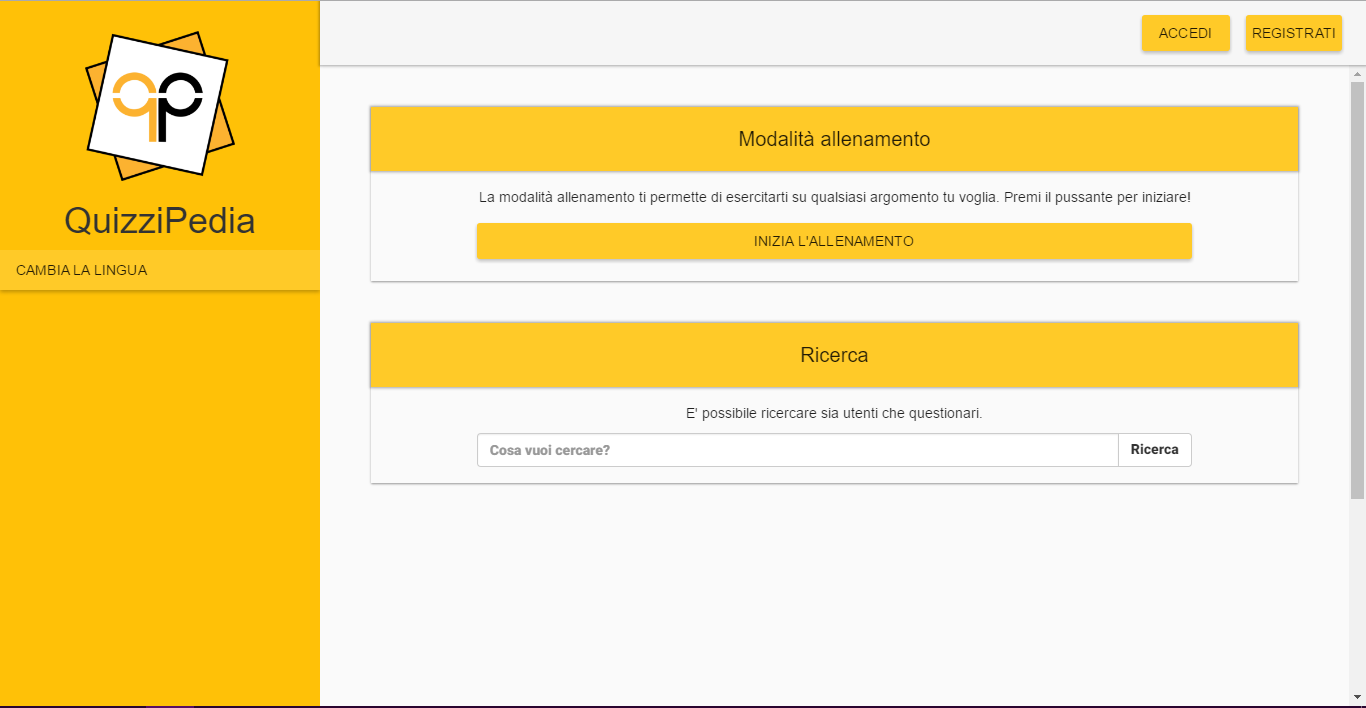
\includegraphics[scale=0.43]{img/homePage.png}
	\caption{Home Page}
\end{figure}
\FloatBarrier

L'Home Page di QuizziPedia presenta all'utente non ancora registrato le seguenti possibilità di utilizzo:
\begin{itemize}
	\item Registrazione;
	\item Autenticazione;
	\item Modalità allenamento;
	\item Ricerca utenti e questionari.
\end{itemize}
Le funzionalità \textit{Modalità allenamento} e \textit{Ricerca utenti e questionari} non necessitano di iscrizione al servizio, perciò l'utente non autenticato sarà libero di allenarsi in uno degli argomenti proposti e di ricercare i questionari e gli utenti presenti nel sistema.